%
% -Consider removing sections on Dogbert
% -Checking conditions here is tedious and in some cases wrong:
%		-why the absolute values in the residuals?
%		-consider creating your own plots to verify residuals
%		-Checking linearity of outcome w.r.t. to predictor variables
%
%





% Uncomment this to make slides with overlays:
%\documentclass[slides]{beamer}

% Uncomment these (but comment the above \documentclass line) to make handouts:
\documentclass[handout]{beamer}

% Uncomment these to have more than one slide per page
%\usepackage{pgfpages}
%\pgfpagesuselayout{2 on 1}[border shrink=5mm]
%\pgfpageslogicalpageoptions{1}{border code=\pgfusepath{stroke}}
%\pgfpageslogicalpageoptions{2}{border code=\pgfusepath{stroke}}

\usepackage[]{graphicx, color, hyperref}

\mode<presentation>
{
	%\usetheme[secheader]{Boadilla}
	%\usecolortheme[rgb={.835, .102,.169}]{structure}  
	\usetheme[width= 0cm]{Goettingen}
	%\setbeamercovered{transparent}
}
\setbeamertemplate{navigation symbols}{}
\setbeamertemplate{footline}[frame number]

\definecolor{blue2}{rgb}{0.278,0.278,0.729} 
\newcommand{\blue}[1]{\textcolor{blue2}{#1}}
\newcommand{\white}[1]{\textcolor{white}{#1}}
\newcommand{\red}[1]{\textcolor{red}{#1}}
\newcommand{\xbar}{\overline{x}}
\newcommand{\ybar}{\overline{y}}
\newcommand{\phat}{\widehat{p}}
\newcommand{\prob}{\mbox{Pr}}
\newcommand{\E}{\mathbb{E}}
\newcommand{\Var}{\mbox{Var}}
\newcommand{\cp}{\oplus}
\newcommand{\cm}{\circleddash}


\title{Lecture 27: Model Selection + Multiple Regression Conditions}
\author{Chapter 8.2-8.3}
\date{}


\begin{document}
%------------------------------------------------------------------------------
\begin{frame}
\titlepage
\end{frame}
%------------------------------------------------------------------------------


%------------------------------------------------------------------------------
\begin{frame}[fragile]
\frametitle{Question for Today}
Recall the Mario Kart analysis

\begin{small}
\begin{verbatim}
Coefficients:
              Estimate Std. Error t value Pr(>|t|)    
(Intercept)      41.34       1.71   24.15  < 2e-16 ***
condused         -5.13       1.05   -4.88 2.91e-06 ***
stockPhotoyes     1.08       1.06    1.02    0.308    
duration         -0.03       0.19   -0.14    0.888    
wheels            7.29       0.55   13.13  < 2e-16 ***
---

Residual standard error: 4.901 on 136 degrees of freedom
Multiple R-squared:  0.719,	Adjusted R-squared:  0.7108 
\end{verbatim}
\end{small}

\end{frame}
%------------------------------------------------------------------------------


%------------------------------------------------------------------------------
\begin{frame}[fragile]
\frametitle{Question for Today}

%
% Comment this
%
%This is the \blue{full model}:  every explanatory variable provided is included.
%
%\pause\vspace{0.5cm}
%
%Recall Occam's Razor: \blue{all other things being equal, simpler is better}.  
%
%\pause\vspace{0.5cm}
%
%In our case:  simpler = less predictor variables included in the model.
%
%\pause\vspace{0.5cm}
%
%The act of choosing which predictor variables to include in your model is \blue{model selection}.

\end{frame}
%------------------------------------------------------------------------------


%------------------------------------------------------------------------------
\begin{frame}[fragile]
\frametitle{Two Common Strategies}

There are two \blue{stepwise regression} methods that add/subtract one variable at a time:
\begin{itemize}
\item Backward Elimination
\item Forward Selection
\end{itemize}

\pause
\vspace{0.5cm}

The criteria used will be $p$-values.  

\end{frame}
%------------------------------------------------------------------------------


%------------------------------------------------------------------------------
\begin{frame}[fragile]
\frametitle{Backward Elimination}

%
% Comment this
%
%\begin{enumerate}
%\item Start with the \blue{full model}
%\pause\item While there still exists statistically non-significant variables
%\begin{enumerate}
%\item Identify the variable with the largest p-value and drop it
%\item Refit the model
%\end{enumerate}
%\pause\item Report model once there are no more non-significant variables
%\end{enumerate}

\end{frame}
%------------------------------------------------------------------------------


%------------------------------------------------------------------------------
\begin{frame}[fragile]
\frametitle{Backward Elimination}
Starting here:

\begin{table}[ht]
\centering
\begin{tabular}{r|rrrr}
  \hline
 & Estimate & Std. Error & t value & Pr($>$$|$t$|$) \\ 
  \hline
(Intercept) & 41.3415 & 1.7117 & 24.15 & 0.0000 \\ 
  {\tt cond\_used} & -5.1306 & 1.0511 & -4.88 & 0.0000 \\ 
  {\tt stockPhotoyes} & 1.0803 & 1.0568 & 1.02 & 0.3085 \\ 
  {\tt duration} & -0.0268 & 0.1904 & -0.14 & 0.8882 \\ 
  {\tt wheels} & 7.2852 & 0.5547 & 13.13 & 0.0000 \\ 
   \hline
\end{tabular}
\end{table}

\end{frame}
%------------------------------------------------------------------------------


%------------------------------------------------------------------------------
\begin{frame}[fragile]
\frametitle{Backward Elimination}
Drop {\tt duration}.

\begin{table}[ht]
\centering
\begin{tabular}{r|rrrr}
  \hline
 & Estimate & Std. Error & t value & Pr($>$$|$t$|$) \\ 
  \hline
(Intercept) & 41.3415 & 1.7117 & 24.15 & 0.0000 \\ 
  {\tt cond\_used} & -5.1306 & 1.0511 & -4.88 & 0.0000 \\ 
  {\tt stockPhotoyes} & 1.0803 & 1.0568 & 1.02 & 0.3085 \\ 
  \blue{{\tt duration}} & \blue{-0.0268} & \blue{0.1904} & \blue{-0.14} & \blue{0.8882} \\ 
  {\tt wheels} & 7.2852 & 0.5547 & 13.13 & 0.0000 \\ 
   \hline
\end{tabular}
\end{table}

\end{frame}
%------------------------------------------------------------------------------


%------------------------------------------------------------------------------
\begin{frame}[fragile]
\frametitle{Backward Elimination}
Drop {\tt stockPhotoyes}.

\begin{table}[ht]
\centering
\begin{tabular}{rrrrr}
  \hline
 & Estimate & Std. Error & t value & Pr($>$$|$t$|$) \\ 
  \hline
(Intercept) & 41.2245 & 1.4911 & 27.65 & 0.0000 \\ 
  {\tt cond\_used} & -5.1763 & 0.9961 & -5.20 & 0.0000 \\ 
  \blue{{\tt stockPhotoyes}} & \blue{1.1177} & \blue{1.0192} & \blue{1.10} & \blue{0.2747} \\ 
  {\tt wheels} & 7.2984 & 0.5448 & 13.40 & 0.0000 \\ 
   \hline
\end{tabular}
\end{table}

\end{frame}
%------------------------------------------------------------------------------


%------------------------------------------------------------------------------
\begin{frame}[fragile]
\frametitle{Backward Elimination}
Done.

\begin{table}[ht]
\centering
\begin{tabular}{rrrrr}
  \hline
 & Estimate & Std. Error & t value & Pr($>$$|$t$|$) \\ 
  \hline
(Intercept) & 42.3698 & 1.0651 & 39.78 & 0.0000 \\ 
  {\tt cond\_used} & -5.5848 & 0.9245 & -6.04 & 0.0000 \\ 
  {\tt wheels} & 7.2328 & 0.5419 & 13.35 & 0.0000 \\ 
   \hline
\end{tabular}
\end{table}
 

\end{frame}
%------------------------------------------------------------------------------


%------------------------------------------------------------------------------
\begin{frame}[fragile]
\frametitle{Forward Selection}

%
% Comment this
%
%\begin{enumerate}
%\item Start with the model with no variables
%\pause\item Fit all models with one possible additional variable
%\pause\item Add the additional variable with the smallest p-value if its significant
%\pause\item Repeat steps 2 and 3 until there are no significant additional variables.  
%\end{enumerate}

\end{frame}
%------------------------------------------------------------------------------



%------------------------------------------------------------------------------
\begin{frame}[fragile]
\frametitle{Criticisms of the Techniques}

Critics regard stepwise regression as \blue{data dredging}, where intense computation is used as a substitute for subject area expertise when deciding on a model.  

\pause
\vspace{0.5cm}

\blue{Data mining} involves automatically testing huge numbers of hypotheses about a single data set by exhaustively searching for combinations of variables that might show a correlation.

\end{frame}
%------------------------------------------------------------------------------


%------------------------------------------------------------------------------
\begin{frame}[fragile]
\frametitle{Criticisms of the Techniques}
\begin{center}

\includegraphics[width=\textwidth]{figure/dilbert.png}
\end{center}
\end{frame}
%------------------------------------------------------------------------------


%------------------------------------------------------------------------------
\begin{frame}[fragile]
\frametitle{Assumptions of Multiple Regression}

%
% Comment this
%
%\begin{itemize}
%\item The residuals $e_i$ of the model 
%\begin{itemize}
%\pause\item are nearly normal
%\pause\item have nearly constant variance
%\pause\item are independent
%\end{itemize}
%\pause\item Each variable is linearly related to the outcome
%\pause\item No pattern in residuals relative to dependent variables.  
%\end{itemize}

\end{frame}
%------------------------------------------------------------------------------


%------------------------------------------------------------------------------
\begin{frame}[fragile]
\frametitle{Example Model}
We investigate plots for the following model:
\[
\widehat{{\tt price}} = b_0 + b_1 \times {\tt cond\_new} + b_2 \times {\tt wheels}
\]

%\begin{itemize}
%\pause\item Normal probability plot of residuals
%\pause\item Absolute values of residuals against fitted values: look for non-constant variance
%\pause\item Residuals against each predictor variable
%\end{itemize}

\end{frame}
%------------------------------------------------------------------------------


%------------------------------------------------------------------------------
\begin{frame}[fragile]
\frametitle{Normal Probability Plot of Residuals}

\begin{center}
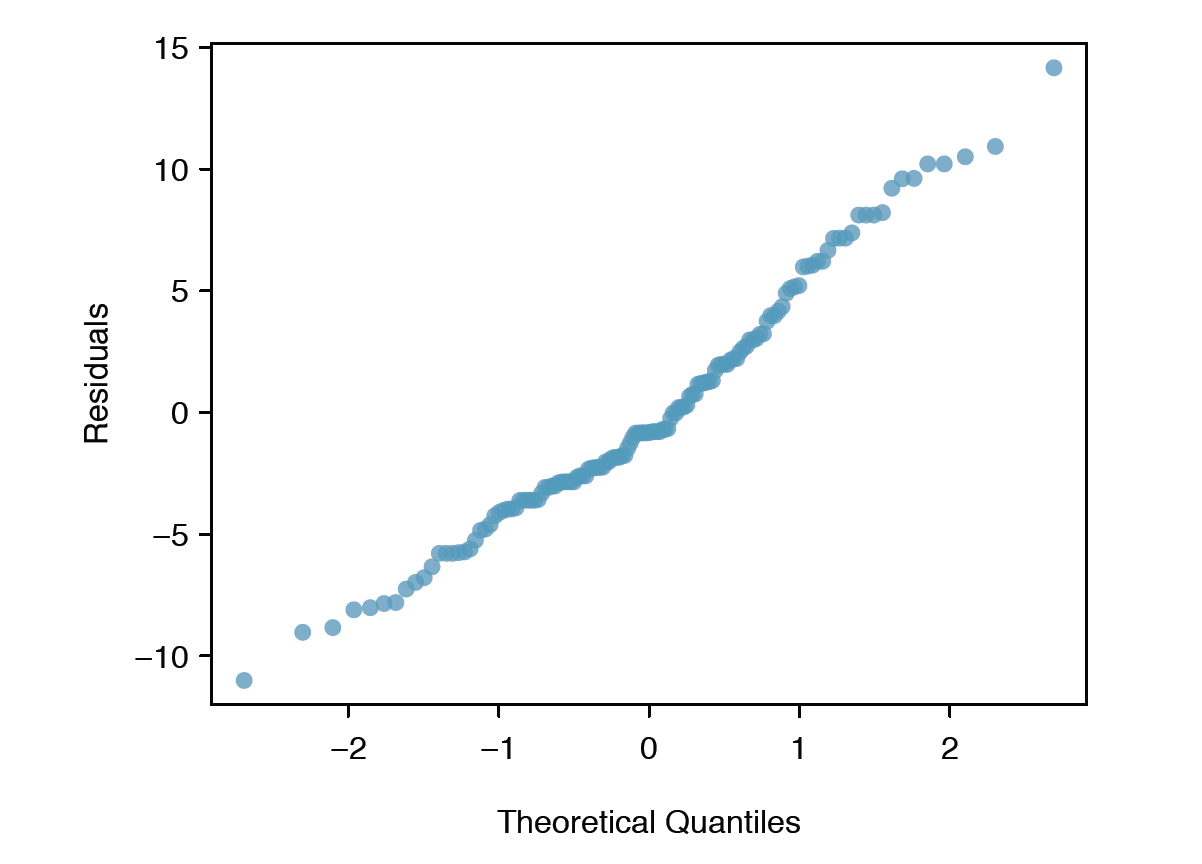
\includegraphics[width=\textwidth]{figure/norm_prob_plot.png}
\end{center}

\end{frame}
%------------------------------------------------------------------------------


%------------------------------------------------------------------------------
\begin{frame}[fragile]
\frametitle{Absolute Values of Residuals Against Fitted Values}

\begin{center}
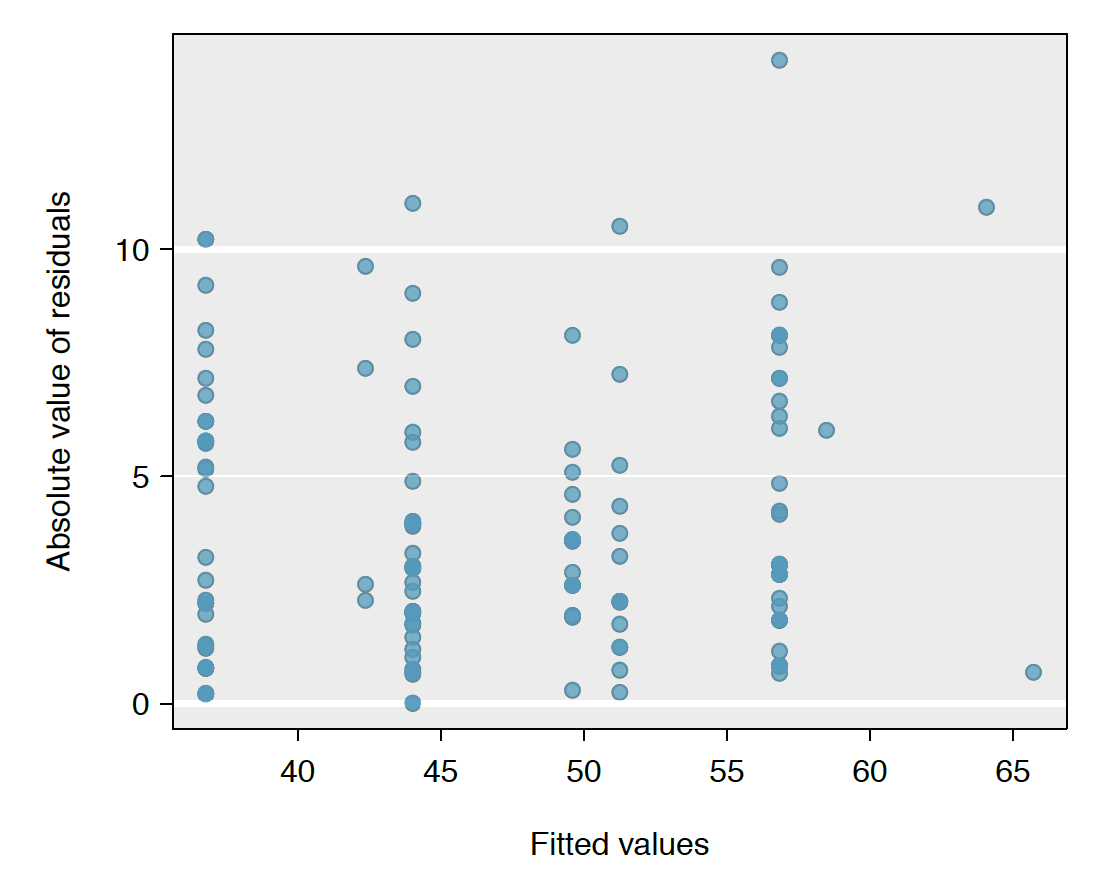
\includegraphics[width=0.8\textwidth]{figure/abs_value.png}
\end{center}

\end{frame}
%------------------------------------------------------------------------------


%------------------------------------------------------------------------------
\begin{frame}[fragile]
\frametitle{Residuals Against Each Predictor Variable: Condition}

\begin{center}
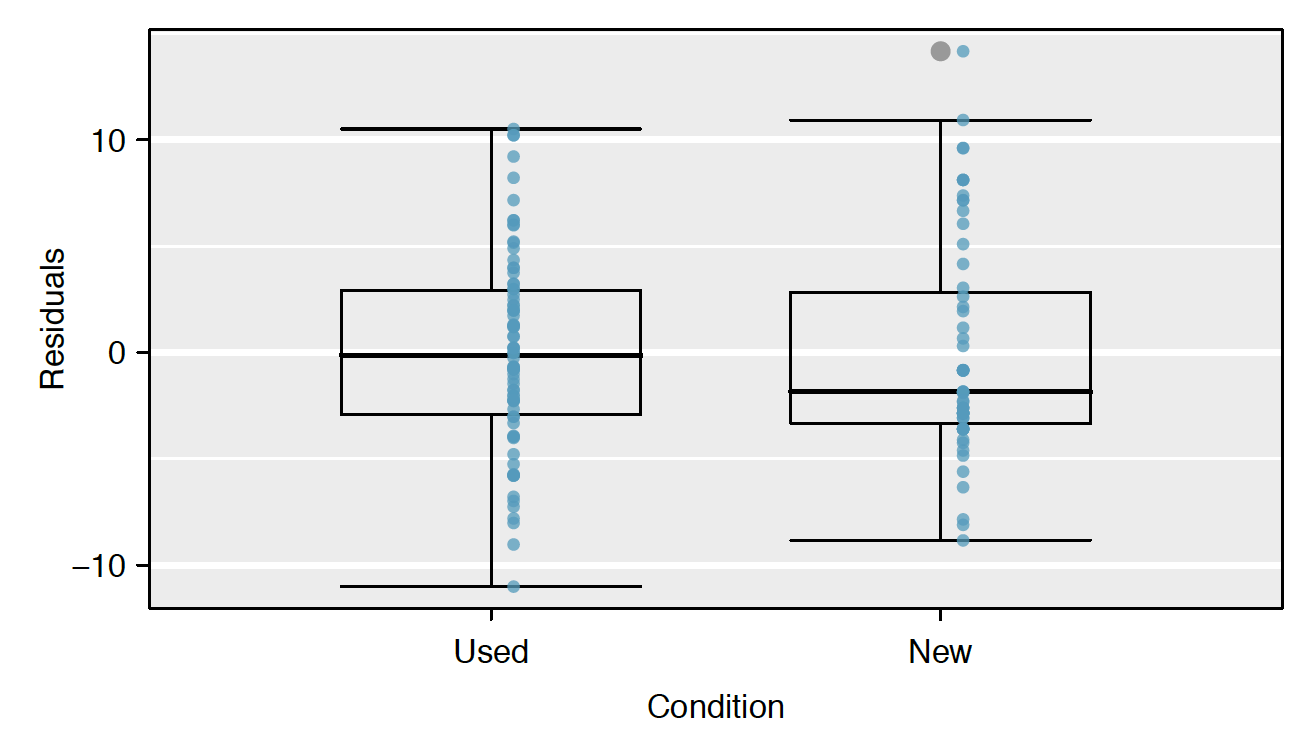
\includegraphics[width=0.8\textwidth]{figure/pred1.png}
\end{center}

\end{frame}
%------------------------------------------------------------------------------


%------------------------------------------------------------------------------
\begin{frame}[fragile]
\frametitle{Residuals Against Each Predictor Variable: Wheels}

\begin{center}
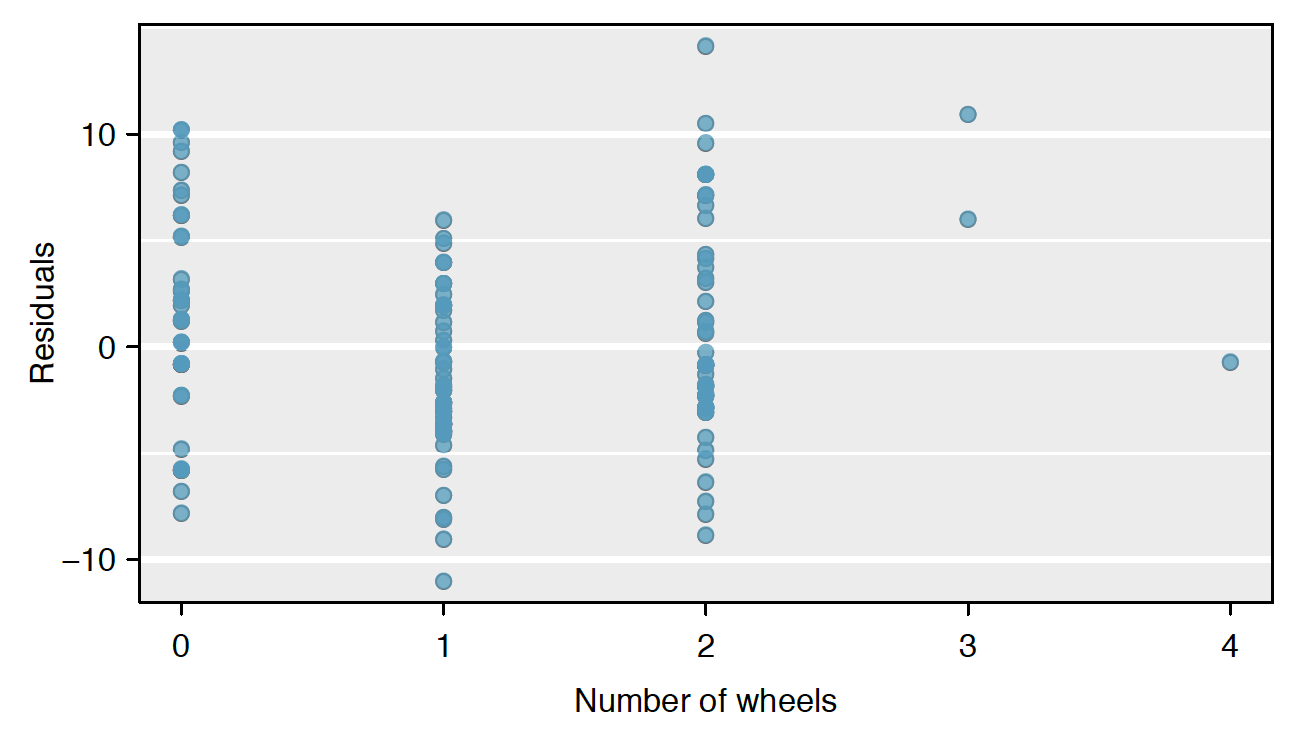
\includegraphics[width=0.8\textwidth]{figure/pred2.png}
\end{center}

\end{frame}
%------------------------------------------------------------------------------


%%------------------------------------------------------------------------------
%\begin{frame}[fragile]
%\frametitle{George E.P. Box}
%There was a famous statistician named Box
%\begin{center}
%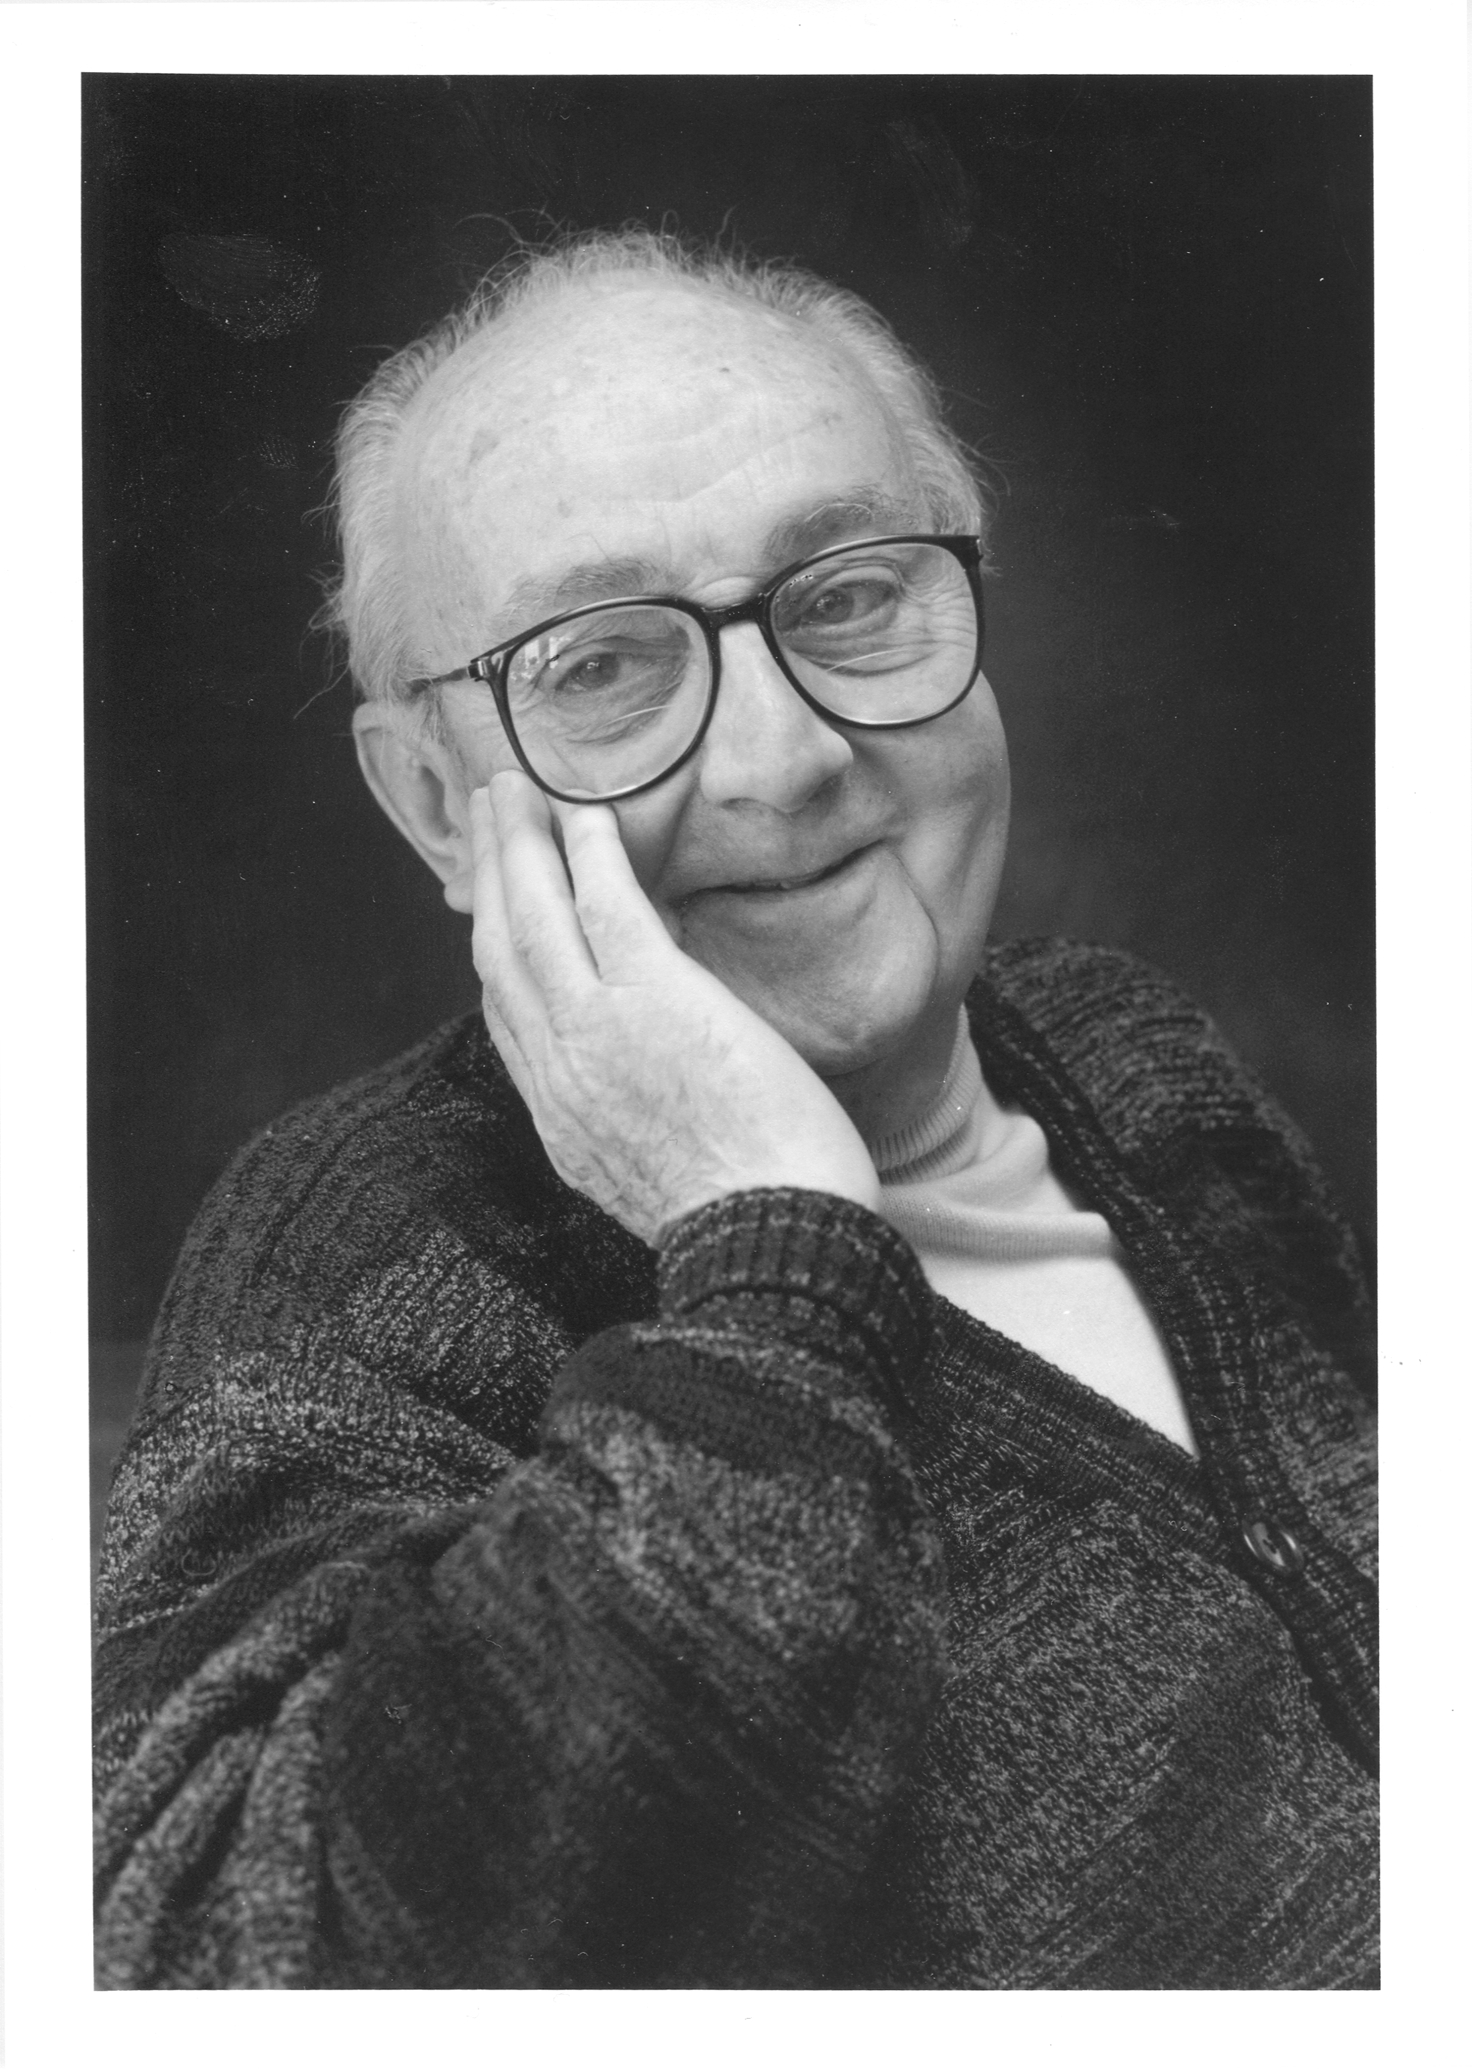
\includegraphics[height=0.5\textheight]{figure/GeorgeEPBox.jpg}
%\end{center}
%famous for the Box/Cox Transformation.  
%\end{frame}
%%------------------------------------------------------------------------------
%
%
%%------------------------------------------------------------------------------
%\begin{frame}[fragile]
%\frametitle{George E.P. Box's Famous Quote}
%
%\blue{``All models are wrong, but some are useful.''}
%
%\end{frame}
%%------------------------------------------------------------------------------
%
%
%%------------------------------------------------------------------------------
%\begin{frame}[fragile]
%\frametitle{Caution}
%
%We can tolerate a little leeway with model assumptions, but when they are grossly violated we have to be skeptical of any confidence intervals/$p$-values.  If model assumptions are clearly violated
%\pause
%\begin{itemize}
%\item consider a new model
%\item get the assistance of someone who can help
%\end{itemize}
%
%\end{frame}
%%------------------------------------------------------------------------------


%------------------------------------------------------------------------------
\begin{frame}[fragile]
\frametitle{Next Time}

What if the outcome variable is not numerical, but rather a \blue{yes/no} response variable?

\pause \begin{itemize}
\item Was an email spam or not?
\item Will someone develop cancer or not?
\item Is a person female?
\end{itemize}

\pause We use \blue{logistic regression}.  

\end{frame}
%------------------------------------------------------------------------------


\end{document}




















%------------------------------------------------------------------------------
\begin{frame}[fragile]
\frametitle{Analysis in Real Life}

My friend JoAnne is a PhD student in Sociology studying the National Parks system.  She fits a multiple regression model where:
\begin{itemize}
\pause\item \blue{data}: results of a government funded survey
\pause\item \blue{outcome variable}: level of support increasing funding for the National parks
\pause\item \blue{predictor variables} include 
\begin{itemize}
\item typical demographic info
\item other info like education, income, etc.
\end{itemize}
\end{itemize}
\end{frame}
%------------------------------------------------------------------------------


%------------------------------------------------------------------------------
\begin{frame}
\frametitle{Missing Data}

One problem she was having was a lot of the income data were \blue{missing data}.  

\pause\vspace{0.25cm}

Her advisor suggested using the \blue{multiple imputation} method, which attempts to \blue{fill in} these missing values.  She doesn't understand this method, nor do I very well.  

\pause\vspace{0.25cm}

The income variable was 3-level categorical, so a summary of her data was:
\begin{itemize}
\item $n$ in low-income
\item $n$ in medium-income
\item $n$ in high-income
\item $n$ of missing data
\end{itemize}

\end{frame}
%------------------------------------------------------------------------------


%------------------------------------------------------------------------------
\begin{frame}
\frametitle{Missing Data}

But then I asked her \blue{were a lot of the other variables missing as well}?  She said no.  

\pause\vspace{0.5cm}

So I surmised that the data wasn't ``missing'' because of clerical errors, people forgetting to enter the values, etc.  

\pause\vspace{0.5cm}

Rather, these people were deliberately \blue{not volunteering} this information.

\end{frame}
%------------------------------------------------------------------------------


%------------------------------------------------------------------------------
\begin{frame}
\frametitle{Missing Data}

Maybe they are a class of people who have privacy concerns?  Maybe this has an impact on their ultimate support of the National Parks?  So instead of looking at income as follows:

\pause
\begin{itemize}
\item $n$ in low-income
\item $n$ in medium-income
\item $n$ in high-income
\item \blue{$n$ of missing data}
\end{itemize}

\pause
look at it as
\begin{itemize}
\item $n$ in low-income
\item $n$ in medium-income
\item $n$ in high-income
\item \blue{$n$ who are sensitive about reporting income}
\end{itemize}

\end{frame}
%------------------------------------------------------------------------------


%------------------------------------------------------------------------------
\begin{frame}
\frametitle{Lesson}

The moral of the story:  statistics is just a tool that always comes \blue{second} to the scientific question of interest and the data at hand.

\pause\vspace{0.5cm}

Rather than using fancy statistical machinery that we didn't understand, we thought about the question/data and found a work around.  

\pause\vspace{0.5cm}

In this case, the missing data was a blessing in disguise:  we found a work around that lead to a new model that might potentially yield better inference than the original model.

\end{frame}
%------------------------------------------------------------------------------




